% !TEX root = thesis-journal.tex
\section{Constructs and Data Collection Methods}
\label{chap:meth}
%Before we dive into our actual studies of the effect of socio-technical congruence and its use to form recommendations, we present the overall roadmap for this thesis (Section~\ref{c5:sec:roadmap}) and some common definitions (Section~\ref{c5:sec:definitions}) and constructs (Section~\ref{c5:sec:constructs}) that we use for the remainder of the thesis.
%Furthermore, we also will discuss the general approach to the data collection methods employed (Section~\ref{c5:sec:datacollection}).

%\begin{figure}[h!]
%\centering
%\includegraphics[height=.9\textheight]{./figures/roadmap}
%\caption{What chapter addresses which research questions in relation to our approach to improve social interactions among software developers.}
%\label{fig:roadmap}
%\end{figure}

%\subsection{Methodology Roadmap}
%\label{c5:sec:roadmap}
%In this section we discuss the methods we apply to answer the research questions presented in Chapter~\ref{chap:bg}.
%Figure~\ref{fig:roadmap} depicts the relationship between the research questions and the contribution of this thesis, an approach to improve social interactions among developers by characterizing the quality of interactions by the build outcome of the related build.
%Research questions~1.1 and~1.2 discussed in Chapters~\ref{chap:soc-net} and~\ref{chap:stc-net2} motivate the approach.
%Research questions~2.1 and~2.3 (Chapters~\ref{chap:stc-net} and~\ref{chap:actionable}) explore whether socio-technical networks can be used to form recommendations that can prevent build failures, whereas research question~2.2 inquires in Chapter~\ref{chap:talk} whether such recommendations are acceptable by developers.
%
%\subsubsection{Research Question 1.1}
%%Motivation
%\begin{itemize}
%  \item\textbf{RQ 1.1:} Do Social Networks influence build success? (Chapter~\ref{chap:soc-net})
%\end{itemize}
%The thesis goal is to design an approach that is able to improve the social interactions in the form of communication among software developers.
%As a first step we need to establish if the communication among software developers has an influence on the build success.
%
%%Data Source
%We have access to the development repositories used by the IBM Rational Team Concert development team such as their source code management system, communication repositories in the form of work item discussions, and their build results.
%All these artifacts are linked together in a way that we can trace from the build result which changes went into the build and which work items a change is meant to implement.
%
%%Methods
%Using this information we can construct social networks from all the work items that are related to builds.
%These networks are then described using social network metric and form the input for machine learning algorithms to predict whether a build based on these metrics is more likely to fail or succeed.
%
%%Expected results
%Via this machine learning approach we want to establish a connection between a build's social network and its outcome. 
%If we are able to predict the build outcome more accurately than by simply guessing, using the likelihood for a build failure, we demonstrated that there is a statistical relationship between build outcome and social networks.
%Thus, this result forms the first evidence that manipulating the social network might yield a positive effect on build success.
%
%\subsubsection{Research Question 1.2}
%\begin{itemize}
%  \item\textbf{RQ 1.2:} Does Socio-Technical Networks influence build success? (Chapter~\ref{chap:stc-net2})
%\end{itemize}
%
%%Motivation
%Knowing that a social network can influence the success of the corresponding build leads us to the question of how networks should be manipulated to improve the likelihood for a build to succeed.
%Therefore, we explore the relationship between socio-technical networks generally and gaps within that networks, with a gap being formed by two developers that share a technical dependencies but did not communicate about work related to the build of interest, and build success.
%%Data Source
%Similarly to the previous research question, we base the analysis on the same data set, as it allows us to directly infer technical relationships among developers related to a software build from the changes submitted to the source code management tool.
%We used these changes previously to infer the work items developers used to communicate among each other about the build.
%
%%Methods
%Since the socio-technical networks has two semantically different edges connecting two developer within a network (technical dependencies and communication among developers) we refrain from using social network metrics as they assume only one mode of connection among nodes within a network.
%Instead we investigate the relationship of the socio-technical congruence index and build success as well as focusing on the influence of gaps in the network on build success.
%
%%Expected results
%Via statistical analysis methods such as regression analysis we want to establish a relationship between the existence of gaps within the socio-technical network and build success.
%By addressing this research question we obtain another piece of evidence that let us formulate an approach to recommend actions to increase build success that are specifically alleviating gaps within the socio-technical network by recommending developer to communicate.
%
%\subsubsection{Research Question 2.1}
%\begin{itemize}
%  \item\textbf{RQ 2.1:} Can Socio-Technical Networks be manipulated to increase build success? (Chapter~\ref{chap:stc-net})
%\end{itemize}
%%Motivation
%The previous two research questions enable us to formulate an approach to generate recommendations that are meant to foster communication among developers in order to increase build success.
%This leads to the next step, namely, to explore whether this approach can generate recommendations that bear a statistical relationship to build success.
%
%%Data Source
%With the same data source we used to explore the previous two research questions, we try to relate individual reoccurring gaps in socio-technical networks to build failure.
%%Methods
%Knowing those gaps, or developers that frequently share a technical dependency without communicating with respect to a build that failed we check if adding a social dependency would change the likelihood of a build to fail.
%%Expected results
%We expect to find a number of gaps that when mitigated increase the likelihood of build success.
%
%\subsubsection{Research Question 2.2}
%\begin{itemize}
%  \item\textbf{RQ 2.2:} Do developers accept recommendations based on software changes to increase build success? (Chapter~\ref{chap:talk})
%\end{itemize}
%%Motivation
%Before exploring if the recommendation hold actual value with preventing build failures, we explore if developers would welcome recommendations with respect to changes.
%%Data Source
%Therefore, we joined the development effort of one of the Rational Team Concert development teams as participant observer to get an insight into how the actual developer communicate during their day to day work.
%
%%Methods
%We complement these observations with followup interviews to gain a better understanding of the team dynamics and their discussion topics, since as a project newcomer our work is limited to more basic tasks in contrast to higher level decision making.
%To extend our reach beyond the local team we deployed a questionnaire with the product team at large to gain a better understanding whether the recommendations we would supply can easily be integrated in their typical discussions with fellow developers.
%
%%Expected results
%This study should give us a better understanding of whether developers are discussing individual changes, thus justifying the appropriateness of the level of recommendations.
%Furthermore, we expect to uncover general suggestions on when and how to supply such recommendations as developers might not always be interested in individual changes even if they pose a threat to build success.


%\subsection{Methodology}
The concept of socio-technical congruence shows potential to help make software development more efficient.
Cataldo et al~\cite{cataldo:cscw:2006} demonstrated its relation to productivity, and we show the ability to use socio-technical congruence to predict build outcome.
The concept of socio-technical congruence lends itself to improve software development as it is based on social networks connecting developer on a coordination and technical level.
Because of the concept being based on networks it is possible to manipulate the networks.

Information in developer socio-technical networks can be leveraged to improve coordination in two ways: (1) changing the technical dependencies among developers by refactoring code or the architecture itself  to make such dependencies unnecessary and (2) by engaging developers in interactions about their recent work and therefore creating a coordination edge in the socio-technical network.
In the first phase in our methodology we assessed whether the actual communication structure among software developers has an influence on build success. 

% to justify using  the basis for manipulating the actual coordination to increase build success.
Having found a relationship between developer communication and build success, we followed up by exploring the relationship between socio-technical networks and build success. More specifically we investigated whether missing actual coordination in the face of a coordination needs is related to build failure.


\subsection{Research Questions and Methodology}
We start with investigating the influence of communication among team members in the form of social networks on build success.
%
%
For this purpose we extract social network metrics describing the social network, such as centrality and betweenness,  and build a predictive model to predict build failure.
%
%
Next, we investigate the amount of gaps (unfilled coordination needs) between developers as highlighted by socio-technical networks and the socio-technical networks in the form of socio-technical congruence can be brought into relation with build success.
%
%
A gap in a socio-technical network is formed when two developer that are technically dependant on each other do not co-ordinate their work.
The presence of gaps results in a lower match in the form of gaps to non-gaps.
We then build a regression model that shows the influence of socio-technical congruence on build failure in the presence of other common failure related metrics.
%
%
Therefore Section~\ref{chap:soc-net} and~\ref{chap:stc-net2} investigate the following two research questions respectively:

%[see if you like my suggestions below:]
\begin{itemize}
  \item\textbf{RQ 1.1:} Are properties of Social Networks related to integration success? (Section~\ref{chap:soc-net})
  \item\textbf{RQ 1.2:} Do gaps in Socio-Technical Networks influence build success? (Section~\ref{chap:stc-net2})
\end{itemize}

Having found a relationship between socio-technical networks, especially gaps between coordination and coordination needs with build success, while knowing that communication alone has an effect on build success, we formulate an approach to leverage socio-technical networks (Section~\ref{chap:approach}).
Thus we focus focus on evaluating this approach in two ways:
(1) gathering general statistical evidence that parts of the network can be manipulated to increase build success and
(2) exploring the acceptance of such recommendation based on those manipulations by developers.
Hence, we are guided by the following two research questions:

\begin{itemize}
  \item\textbf{RQ 2.1:} Can closing socio-technical gaps increase build success? (Section~\ref{chap:approach})
  \item\textbf{RQ 2.2:} Do developers accept recommendations based on software changes to increase build success? (Section~\ref{chap:talk})
\end{itemize}

In the following discussion (Section~\ref{chap:disc}) we will highlight how our findings from our research questions supporting the approach we detailed in Section~\ref{chap:approach}.





\subsection{Constructs}
\label{c5:sec:constructs}
From the definitions introduced previously we can derive the three central constructs we work with: (1) the social network connecting communicating and coordinating developers, (2) the technical network connecting developer that are dependent through code artifacts, and (3) the socio-technical network that combines the social and technical network in a meaningful way.
These constructs are important for the three sections that are mining the repository provided by the Rational Team Concert development team (Sections~\ref{chap:soc-net},~\ref{chap:stc-net2}, and~\ref{chap:approach}).

\subsubsection{Social Network}
%\begin{figure}[t]
%\begin{center}
%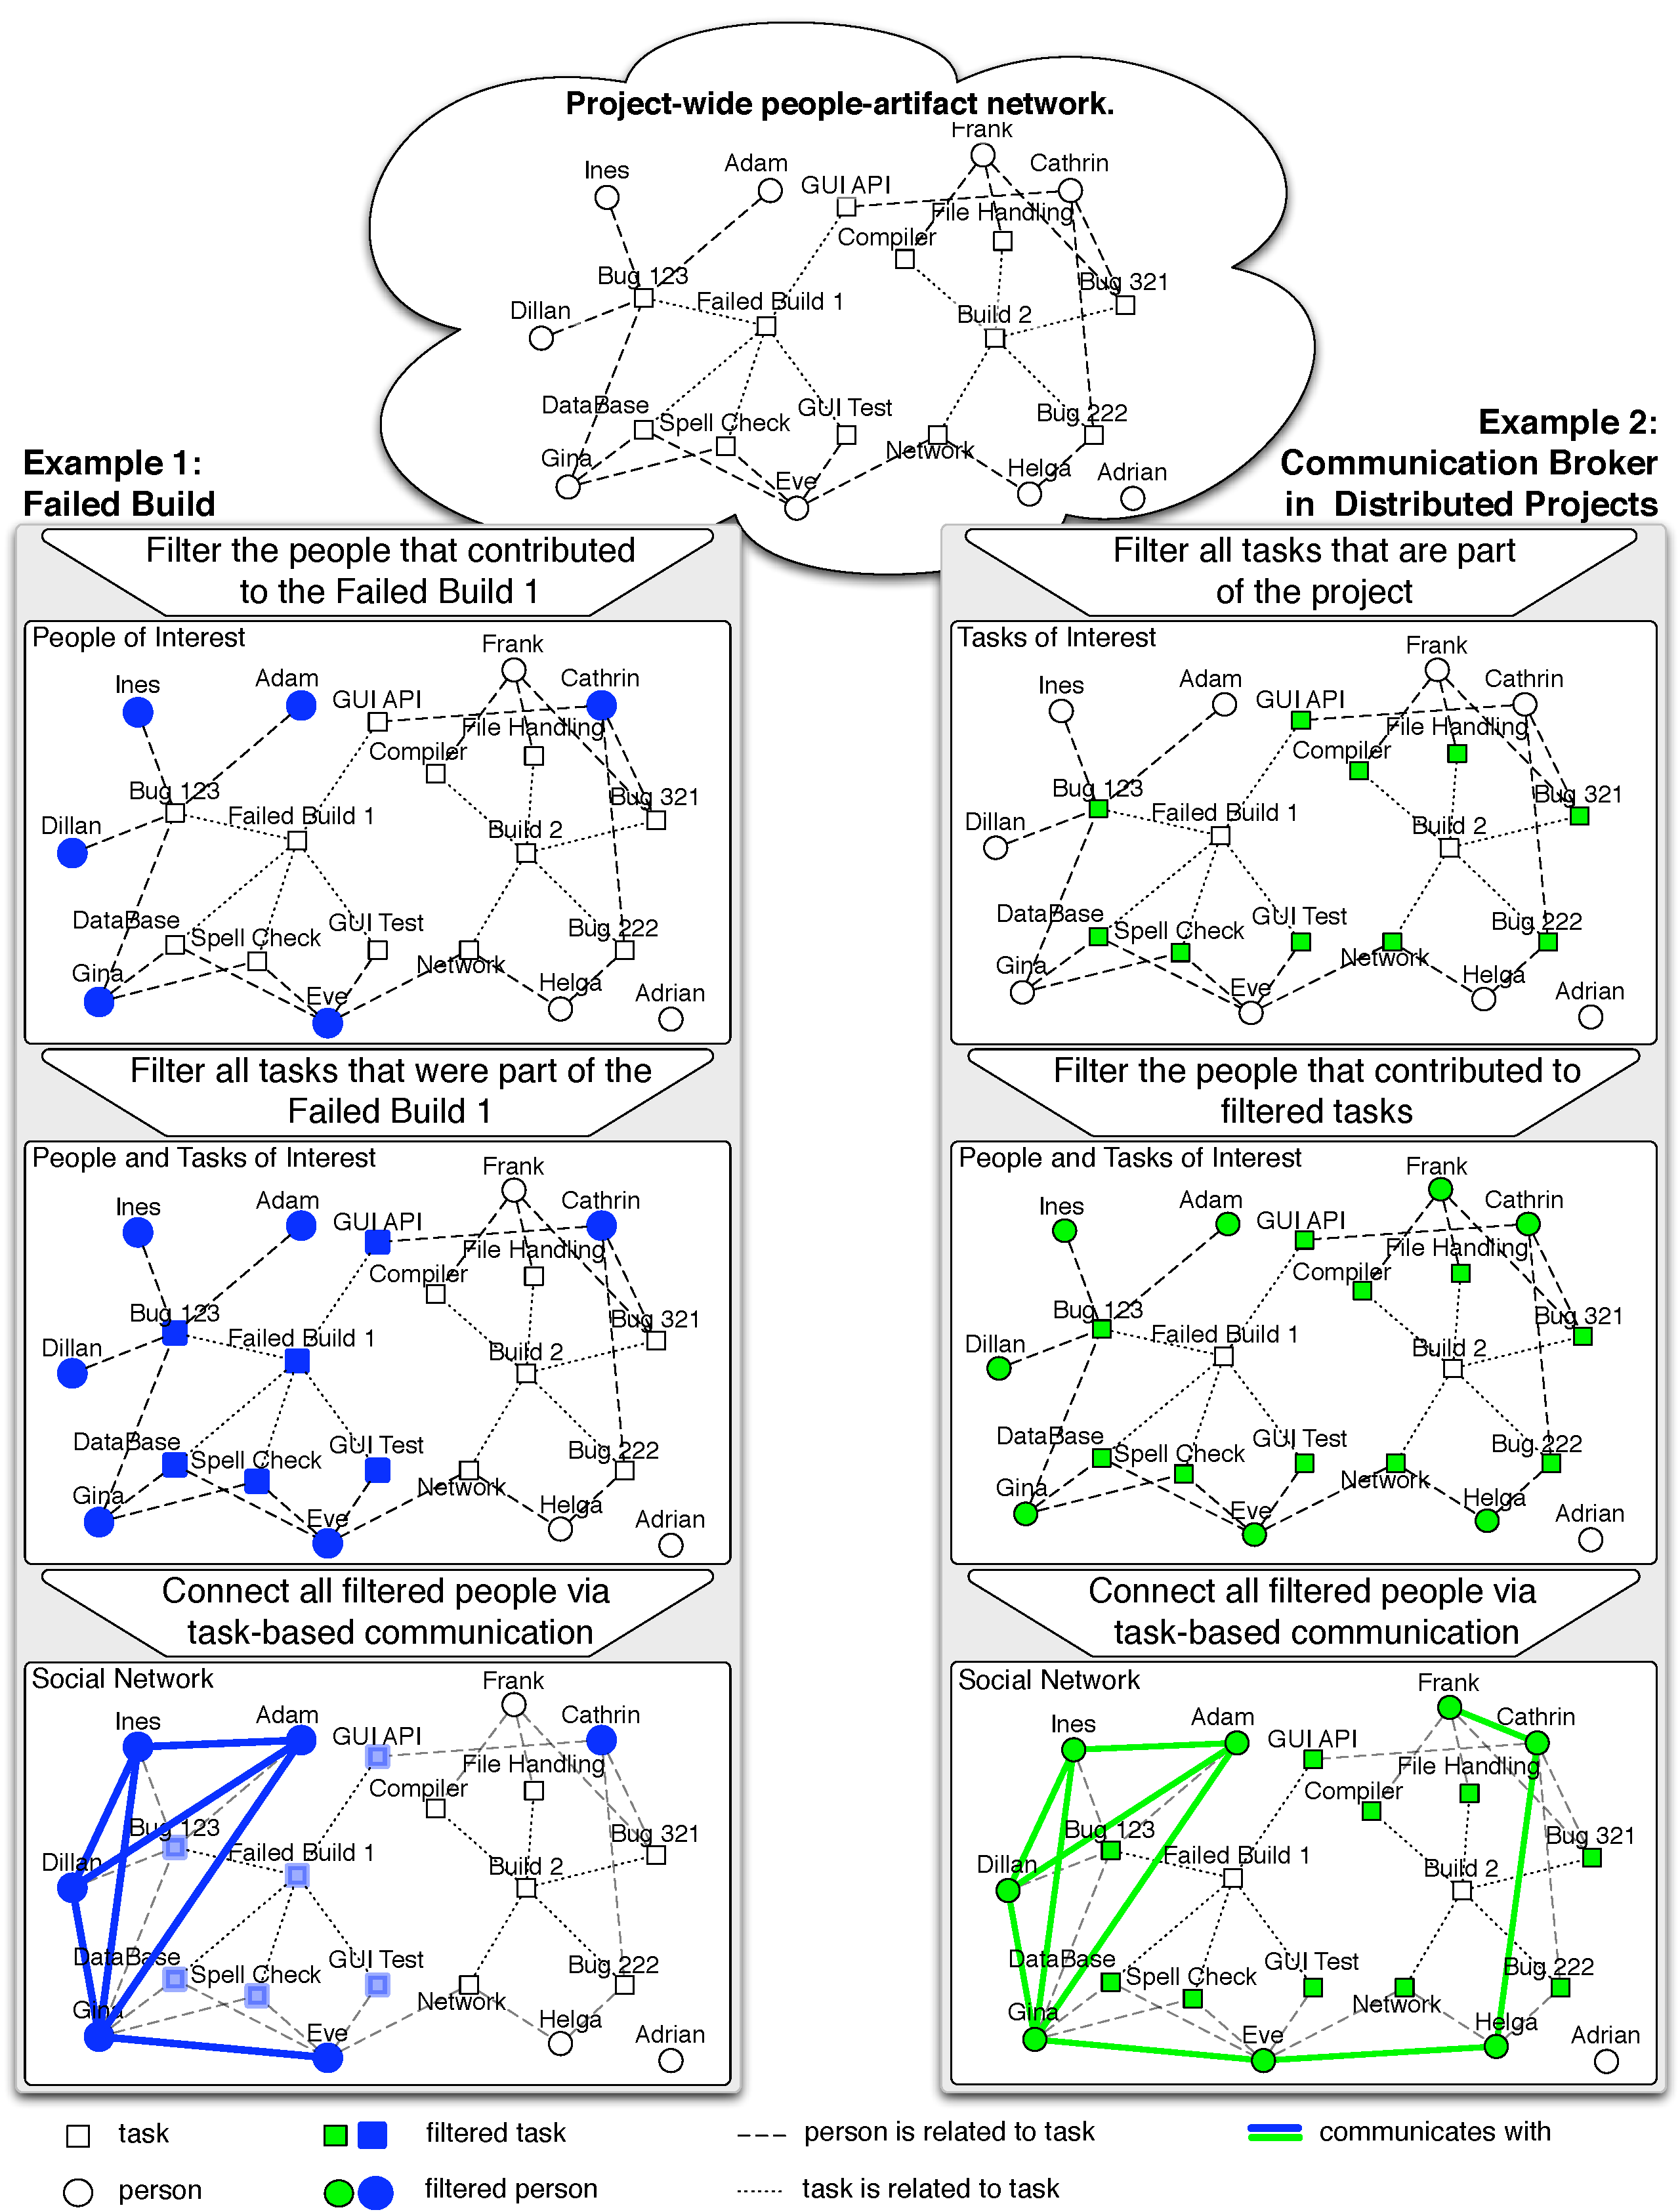
\includegraphics[width=0.8\columnwidth]{./figures/grand_figure}
%\caption{Social network construction examples in our approach}
%\label{fig:network}
%\end{center}
%\end{figure}
A social network is represented as a graph that consist of nodes connected by edges. 
In our approach, the nodes represent people and edges represent task-related communication between these people.

The approach is repository and tool independent and can be applied to any repositories that provide information about people, tasks, technical artifacts, and communication, this includes work, issue, or change management repositories, such as Bugzilla or IBM Rational Team Concert; or source code management systems, such as CVS or IBM Rational Team Concert; or even communication repositories such as email archives.

There are three critical elements that are necessary to construct task-based social networks for a collaboration scope and that need to be mined from software development repositories.
\emph{Project Members}  can be developers, testers, project managers, requirements analysts,
or clients. 
\emph{Work Items} are units of work within the project that may create a need to collaborate and communicate such as a bug report or feature request.
\emph{Work Item Communication} is the information exchanged while completing a work item and is the unique information that allows us to build task-based social networks.


%The data underlying the social network used throughout this thesis are based on work items and their associated discussions.
%In IBM Rational Team Concert each work item has an attached discussion thread were developers can discuss the work item or simply note down their thoughts while working on the work item.
%This means, we would create a link between two developer if they comment together on the same work item to indicate that they are part of the same discussion.
%Note that this sections draws heavily from our work done in collaboration with Timo Wolf, Daniela Damian, Lucas Panjer, and Thanh Nguyen~\cite{wolf:ieee:2009}.

\subsubsection{Technical Network}
%\begin{figure}[th!]
%\centering
%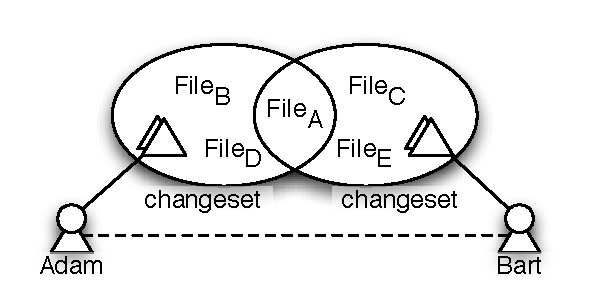
\includegraphics[width=.9\columnwidth]{figures/cochangedfiles}
%\caption{Creating a technical network by connecting developers that changed the same file.}
%\label{fig:construct-tn}
%\end{figure}

% some preamble as in the previous subsection
Building technical networks follows a very similar approach as we described for building social networks.
In fact, the technical network is a social network whose main distinction from the social network described earlier lies in the way edges between nodes are created.
We derive the name of technical network from the way we link developer with each other, namely if they are modifying related source code artifacts.
As in the previous network construction, the construction of the technical network is based on three components.
%
%\begin{itemize}
\emph{Project Members}  can be developers, testers, project managers, requirements analysts,
or clients or in general anyone that modifies software artifacts through change-sets. 
%
\emph{Change-Sets} consist of a number of artifacts that have been modified as well as the modifications themselves.
%
\emph{Software Artifact Relation}  can be defined in several different ways.
For example, in Figure~\ref{fig:construct-tn} Alfred and Bob are related through a technical relationship because they modified the same file.
%\end{itemize}

% Example as shown in the picture
Constructing technical networks therefore follows three steps: (1) we gather all change-sets of interest, (2) identify the relations between artifacts, (3) infer from the change-sets and the relations between the source code artifacts the relation between the artifact owners.
%For example, after we selected the set of change-sets of interest we define the change-sets themselves as the source code artifact and identify the owners of those artifacts.
%Then we infer the relationship between those source code artifacts by relating all change-sets that changes the same source code file.
%And as Figure~\ref{fig:construct-tn} shows this means in the case for Alfred and Bob that they are connected because both own a change-set that modifies the same file.

\subsubsection{Socio-Technical Network}
\begin{figure*}[t!]
%	
  \centering
  \subfloat[Inferring to the build focus relevant change-sets and work items.]{
    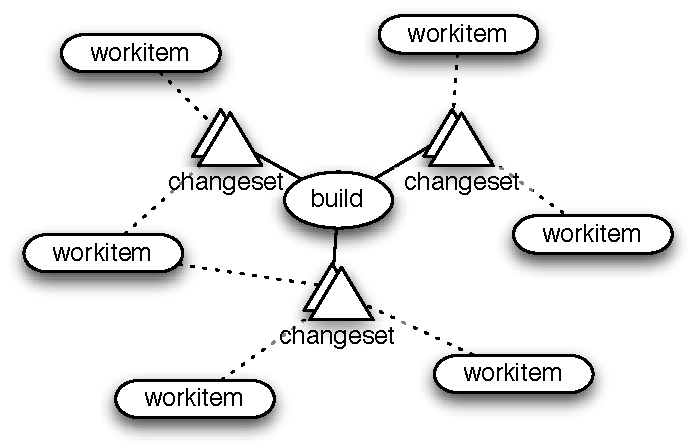
\includegraphics[width=.22\textwidth]{figures/buildworkitem}
    \label{fig:construct-focus}
  }
% 
\hspace{5pt}
  \subfloat[Constructing an social networks from work item communication.]{
	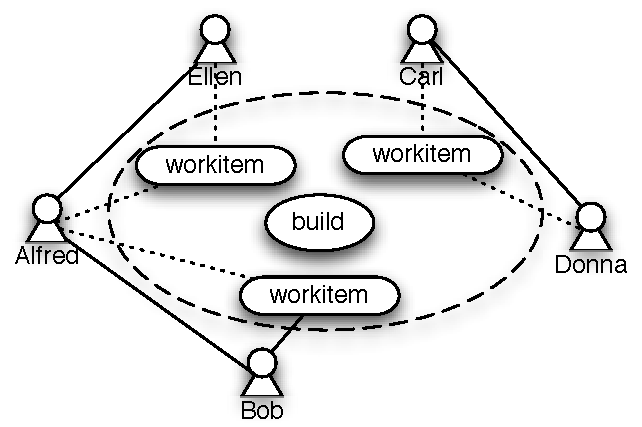
\includegraphics[width=.22\textwidth]{figures/buildsn}
     \label{fig:construct-sn}
  }
\hspace{5pt} 
    \subfloat[Linking developers in a technical networks via change-set overlaps.]{
  	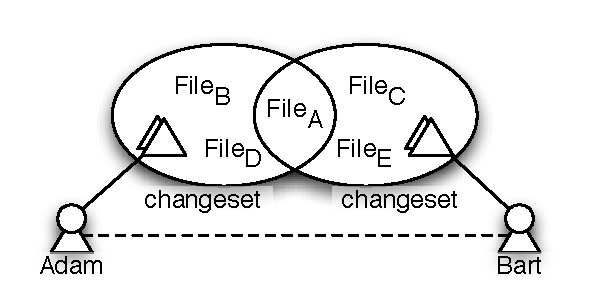
\includegraphics[width=.22\textwidth]{figures/cochangedfiles}
    \label{fig:construct-tn}
  }
\hspace{5pt}
  \subfloat[Combine social and technical networks into a socio-technical network.]{
  	\includegraphics[width=.22\textwidth]{figures/stc-net}
	\label{fig:construct-combine}
  }
  \caption{Constructing socio-technical networks from the repository provided by the IBM Rational Team Concert development team.}
  \label{fig:construct-stc}
\end{figure*}

Socio-Technical networks are a meaningful combination of both social and technical networks.
Selecting this meaningful combination reflects itself in the selection of the work-items in the case of building the social network and selecting the change-sets and their relations in the case of the technical network.
Hence constructing a socio-technical network requires the following four steps:

\begin{enumerate}
\item\textbf{Selecting the Focus} used for the socio-technical network represents the glue that binds the social and technical network into a socio-techncial network. 
This focus also referred to as filter in our earlier publication~\cite{wolf:ieee:2009}, determines the content of the networks.
\item\textbf{Constructing the Social Network} we build social networks from all work items that are relevant to the defined focus.
\item\textbf{Constructing the Technical Network} follows the description of constructing technical networks above with the focus determining the change-sets being used to determine and connect developers in the network.
\item\textbf{Combining Networks} overlays the networks by unifying the set of developers in both networks.
\end{enumerate}

% describe the example in the figure
Figure~\ref{fig:construct-stc} shows an example on how we in our studies of the IBM Rational Team Concert development team used to create socio-technical networks.
In the first step (Figure~\ref{fig:construct-focus}) we set the focus to be a software build which allows us via the change-sets that made it into the build to infer what work items are also represented in said build.
Given the focus, the social network can be constructed using the work items that can be linked to the software build (Figure~\ref{fig:construct-sn}).
Similarly the construction of the technical network relies on the change-sets that went into a build. 
To actually infer edges between developer, we relying on co-changed files within a build as an indicator of work dependency (Figure~\ref{fig:construct-tn}).
Finally, the two networks are combined and yield the socio-technical network shown in Figure~\ref{fig:construct-combine}.

\subsection{Data Collection Methods}
\label{c5:sec:datacollection}
To conduct our research we drew upon multiple data sources.
We employ repository mining techniques to identify larger trends in measurable activities.
In contrast to gain a more in-depth understanding on how developers actually work and deal with interdependencies especially how they would react to certain recommendations and whether they are can be made useful we employ qualitative methods.

\subsubsection{Repository Mining}
Software development usually uses a number of tools to manage information electronically such as version archives and issue trackers.
Additionally to storing source code and tasks/issues, those software repositories can also contain digital communication such as forum and email discussions.

%Repositories can grow to considerable sizes depending on the projects live span and intensity. 
%Therefore, it is often infeasible to manually review the history of a project and it is necessary to employ data-mining techniques to be able to analyze trends.
%Data mining approaches leveraging this wealth of data are one way to easily give back value to the development team without burdening any individual developer with diverting time to other non-automatic data collection instruments.
%technical congruence to generate actionable recommendations.
%In case a developer needs to personally provide a large amount of information manually the overhead generated by a system might outweigh the benefit of recommendations and therefore make the system useless.

We extract information from three different types of repositories: (1) version control, (2) task management, and (3) build engine systems.
The version control supplies us with the knowledge on how developers are connected through their technical work.
The task management supplies us with the information on who communicated with whom with respect to a work item.
And lastly the build engine supplies us with the focus to construct socio-technical networks.

In order to derive socio-technical networks we need to link the different artifact types.
Within IBM Rational Team Concert as illustrated in Figure~\ref{fig:construct-focus} work items are linked to change-sets and change-sets are linked to builds, therefore, establishing the connections needed to construct socio-technical networks with a build as focus.

\subsubsection{Surveys}
To complement the insights we obtained from mining repositories we use surveys.
Surveys are designed iteratively and piloted before deployment, and intended to collect input to enrich and clarify information obtained from the software repositories. 
With each survey we try to minimize the time each developer needs to spend completing them, which usually limits ourselves to focus on closed questions.
We constrain ourselves in this way to minimize the distraction to each individual developer and thus increase the response rate.

Our surveys are deployed through web services to make the collections more convenient to each developer as they are spending most of their times working at a computer enabling them to fill out the survey at their earliest convenience.
Keeping track of a paper version is more cumbersome as they might not easily be returned, especially considering that the development teams we are collaborating with are distributed across different continents.


\subsubsection{Observations}
The next richer and also to the developer more distracting method of data gathering are observations.
Although not necessarily actively interrupting and distracting developer, the act of observing can distract developers and also change their behaviour.
In order to minimize this type of distraction and to mitigate the observer bias, we employed a special form of observation study namely participant observation.
In short we became both an observer and a participant.
%
Being a participant observer has a multitude of advantages:

%\begin{itemize}
\emph{Reciprocity.} By participating in the actual development we can provide value to the development team from the very beginning.
This, in turn, motivates the developers to give us the time we need to conduct other parts of the study, like surveys and interviews.
\emph{Learning the Vocabulary.} Each development project has its own project vocabulary~\cite{espinosa2007:team_knowledge} in order to effectively and clearly communicate. 
Understanding this vocabulary as an outsider is not necessarily easy but very important to make sense of comments and answers supplied in interviews and surveys.
\emph{Understanding the Context.} For example, in one study our observation period coincided with the months prior to a major release. 
% something about the context helping
Because of this closeness of our observation period to a major release we observed mainly activities around integration testing with little coding activity aside from fixing major bugs.

%Although it is easy to ascertain when the next major release of the product is, the effect this has on the developer besides a change in the process is harder to gauge.
%Being part of the development effort allowed us to better understand how developers react to the change in process and better understand their struggles.

\emph{Asking more Meaningful Questions.} A better understanding of the project and how it affects the individual developer as well as understand the vocabulary helps with phrasing better questions.
%Better in the sense of both more meaningful to the developer and in the sense of understandability because they can be phrased using the project vocabulary.
%\end{itemize}

Besides gaining a better understanding of some easily missed or miss-understood intricacies, working together with the developer establishes a trust relationship~\cite{letherbridge:ese2005}.
This trust helps to mitigate observation biases that are introduced by just observing as well as makes developers more forthcoming during interviews and surveys~\cite{letherbridge:ese2005}.
%We were able to join the Rational Team Concert development team as a participant observer mainly due to the convincing argument that we take the place of an intern, thus, contributing to their development effort (Chapter~\ref{chap:talk})

\subsubsection{Interviews}
To further enhance our understanding on how developers view the situation, we employed interviews.
Instead of following a structured interview approach, we opt for a semi-structured interview with a focus on war stories.
War stories~\cite{lutters:ist:2007} ask the interviewee to share memorable stories from work life.
The interviewer than can explore those war stories and help shape the focus of the discussion of those events.
This type of interview comes with two major benefits over structured interviews that follow a set of questions:

%\begin{itemize}
\emph{Focus onto for the interviewee important events.}
Knowing the pain points as they are perceived by the projects participants allows us to focus on important issues.
With prepared questions the focus of the interview might not uncover what is important to the interviewee and thus we might miss areas.
\emph{Better recall of events by interviewee.}
Recall of events of importance is better than of arbitrary events~\cite{lutters:ist:2007}.
This allows us to place more confidence into the reports and answers given by the interviewees.
%\end{itemize}

%The main drawback of using war stories over prepared interview questions in a structured interview framework lies with the loss of focus of the interviews.
By asking the interviewee to tell war stories of memorable events it can be more difficult to gain the insights into a particular area of interest if the war stories veer to far off the topic of interest.
It is therefore necessary that the interviewer has a good understanding of the project and the project language to explore the stories for relevance to topics of interest making it thus more demanding on the side of the interviewer.

% talk about the time of the interviews
%We tried to minimize the interruption to project members as much as possible therefore we limited the time we require for each interview as much as possible.
%Most interviews are aimed at taking 30 minutes with a 30 minute overflow in case a participant is willing to continue the interview.
%Furthermore, we gave the work of the interviewee priority over the interview and assured the interviewees that they could stop the interview anytime they felt that their work needs attention.
%This was especially valuable with a professional development team such as the IBM Rational Team Concert development team as we joined their development effort when they were nearing a major milestone (Chapter~\ref{chap:talk}).










